\providecommand{\main}{..}
\documentclass[\main/main.tex]{subfiles}

\begin{document}
    \justify
    \subsection{Badanie wpływu wartości wag początkowych na szybkość uczenia Adaline}
    \paragraph{}
    Badanie ma na celu zweryfikowanie wpływu wartości wag początkowych na działanie Adaline. Badania przeprowadzone zostały dla unipolarnej funkcji aktywacji oraz unipolarnego zbioru uczącego. Wykorzystano współczynnik uczenia a = 0.05, zakres dopuszczalnego błędu natomiast został ustawiony na 0.08.
    
    \paragraph{}
    Zbadano natomiast następujące przedziały:
    \begin{itemize}
     \item (-1, 1)
     \item (-0.8,  0.8)
     \item (-0.6, 0.6)
     \item (-0.4, 0.4)
     \item (-0.2, 0.2)
     \item (-0.05, 0.05)
     \item (0, 0)
    \end{itemize}
    
    \paragraph{}
    Tak jak zostało to wcześniej wspomniane, prezentowane wyniki są wartościami uśrednionymi, \\hline
    uzyskanymi w skutek wielokrotnego uruchomienia algorytmu i prezentują się one następująco.

    \begin{figure}[H]
    \centering
    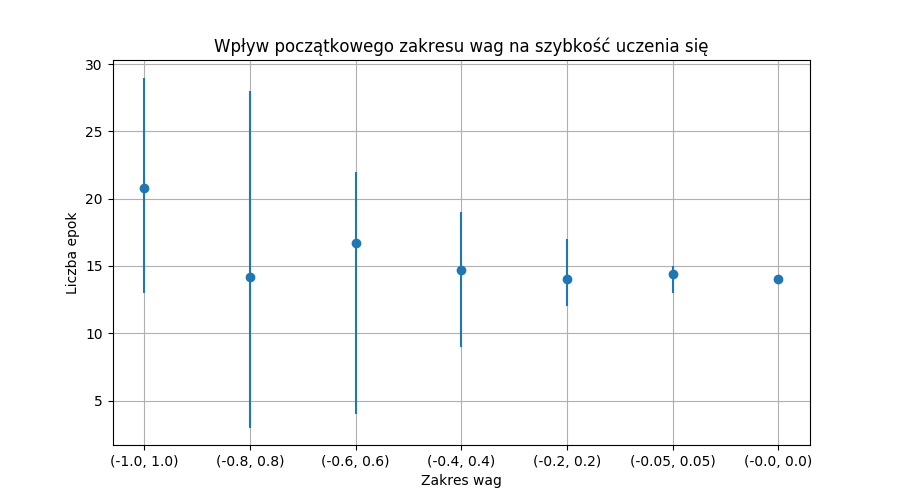
\includegraphics[scale=0.6]{test_weights_Adaline_10}
    \caption{Wyniki badań uzyskane w skutek 10 uruchomień}
    \end{figure}

    \begin{figure}[H]
    \centering
    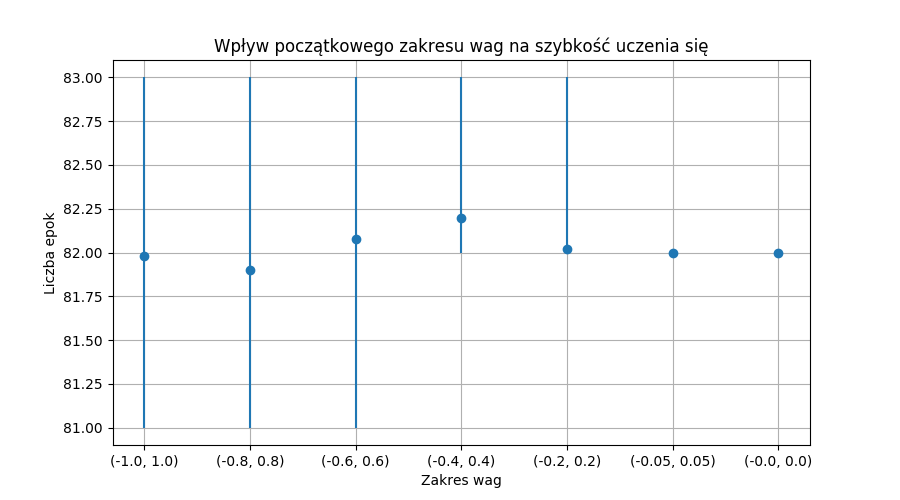
\includegraphics[scale=0.6]{test_weights_Adaline_100}
    \caption{Wyniki badań uzyskane w skutek 100 uruchomień}
    \end{figure}
    
    \paragraph{}
    Można zauważyć, że wyniki całkowicie różnią się od tych uzyskanych przy wykorzystaniu perceptronu prostego. W przypadku Adaline, średnia liczba epok wymaganych do wytrenowania modelu jest praktycznie stała, z niewielkimi odchyłami. Widać jednak, że w przypadku mniejszych przedziałów zmniejsza się różnorodność uzyskanych wyników, jednoznacznie wskazują na to przedziały nieufności. Wyniki te spowodowane są zasadą działania Adaline, który zawsze zmierza to ustalenia tych samych optymalnych wag, niezależnie od wartości wag początkowych. Dodatkowo, w przypadku Adaline, wagi poprawiane są nie o błąd otrzymany w wyniku nałożenia funkcji aktywacji, a całkowite pobudzenie neuronu. Umożliwia to bardziej dokładne aktualizacje wartości wag, co prowadzi do szybszego znalezenia rozwiązania.

    \justify
    \subsection{Badanie wpływu współczynnika uczenia  na szybkość uczenia Adaline}
    \paragraph{}
    Badanie ma na celu określenie wpływu wartości współczynnika uczenia na działanie perceptronu prostego. Badania przeprowadzone zostały dla unipolarnej funkcji aktywacji oraz unipolarnego zbioru uczącego. Przedział wag do badania został wybrany na podstawie poprzednich obserwacji i ma wartość [-0.2, 0.2].
    
    \paragraph{}
    Badania przeprowadzono na następujących wartościach współczynnika.
    \begin{itemize}
    \item 0.01
    \item 0.05
    \item 0.1
    \item 0.2
    \item 0.5
    \item 0.8
    \item 1.0
    \end{itemize}
    
    Wynikiem przeprowadzonych badań są następujące wykresy:
    
    \begin{figure}[H]
    \centering
    \begin{subfigure}{.5\textwidth}
    \centering
    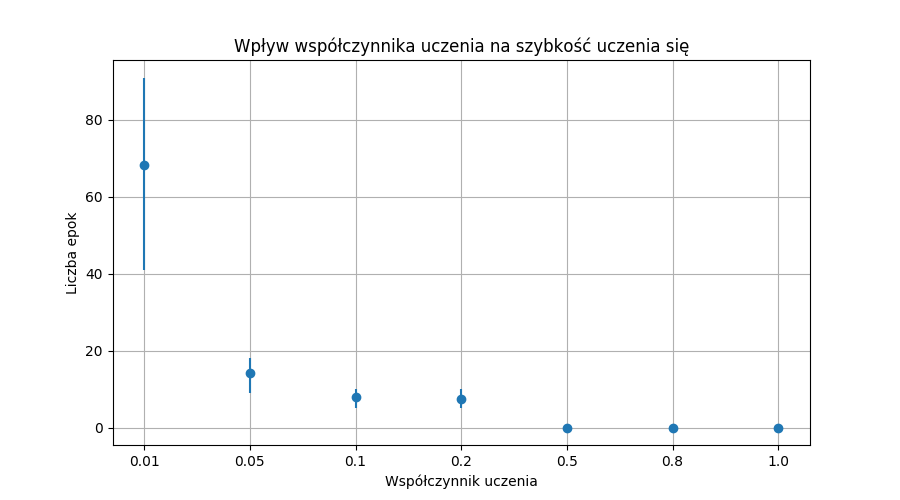
\includegraphics[width=1.1\linewidth]{test_LR_Adaline_100_epochs}
    \caption{Liczba epok w zależności od współczynnika uczenia}
    \label{fig:lr_sp_epochs}
    \end{subfigure}%
    \begin{subfigure}{.5\textwidth}
    \centering
    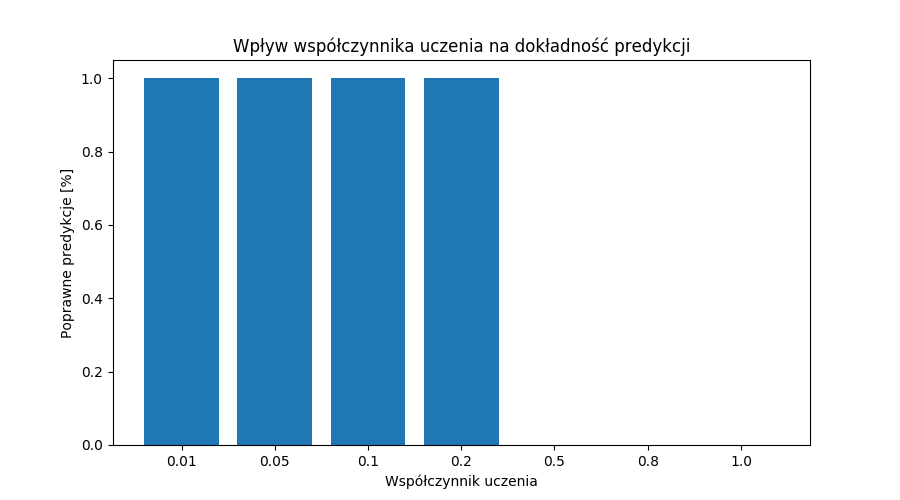
\includegraphics[width=1.1\linewidth]{test_LR_Adaline_100_correctness}
    \caption{Procent prawidłowych predykcji w zależności od współczynnika uczenia}
    \label{fig:lr_sp_correctness}
    \end{subfigure}
    \caption{Wpływ współczynnika uczenia na szybkość i jakość treningu}
    \label{fig:test}
    \end{figure}
    
    \paragraph{}
    Wpływ współczynnika uczenia na szybkość uczenia się Adaline wygląda tak samo jak w przypadku perceptronu prostego. Tak samo jak w przypadku perceptronu prostego, duże wartości współczynnika uczenia uniemożliwiały ukończenie treningu. Można jednak zauważyć, że w przypadku Adaline liczba wymaganych epok dla tej samej wartości współczynnika jest większa. Drugą różnią natomiast jest to, że w przypadku Adaline nie otrzymaliśmy modelu, którego poprawność predykcji była na 50 procent, tak jak w przypadku perceptronu prostego. Głównym tego powodem jest to, że w przypadku dużego współczynnika uczenia, algorytm ciągle wprowadzał zmiany do wag, które powodowały, że błąd średniokwadratowy nigdy nie mógł spaść poniżej zadanej wartości. Oznacza to, że trening nigdy nie mógł się skończyć, a ciągle rosnące wartości błędu prowadziły do otrzymania gigantycznych wag.
    
\end{document}
